\input header.tex
\usepackage{arydshln}


%----------------------------------------------------------------------------------------
%       TITLE PAGE
%----------------------------------------------------------------------------------------
\title[ISDM'24, JISBD, A Coruña]{ISDM'24\\JISBD\\A Coruña\thanks{\url{https://github.com/dsevilla/isdm-jisbd24}}}

\author{Pedro J. Clemente Martín\inst{1}, Diego Sevilla Ruiz\inst{2}}
\institute[]{
\begin{tabular}[h]{cc}
\inst{1} ISIT  &  \inst{2} DITEC \\
Escuela Politécnica &  Facultad de Informática \\
Universidad de Extremadura &  Universidad de Murcia \\
\href{mailto:pjclemente@unex.es}{\textit{pjclemente@unex.es}} &  \href{mailto:dsevilla@um.es}{\textit{dsevilla@um.es}}\\
\end{tabular}}
\date{Junio, 2024}

\begin{document}

\def\insertsectionnumber{\arabic{section}}
\def\insertsubsectionnumber{\arabic{subsection}}

\pgfdeclareimage[width=\paperwidth]{background}{img/portada.jpg}
\usebackgroundtemplate{\tikz\node[inner sep=0,opacity=0.2]{\pgfuseimage{background}};}


\begin{frame}
  \titlepage
\end{frame}

\section{Introducción y bienvenida al taller}

% \begin{frame}
% \frametitle{Bienvenida}

% \end{frame}

\begin{frame}[fragile]
\frametitle{Cargando los datos de easychair}

\begin{lstlisting}
import pandas as pd
df = pd.read_excel('ISDM2024.xlsx',index_col=0,header=0)
df['Authors'] = df['Authors'].str.replace(' and ', ' y ', regex=False)
\end{lstlisting}

\end{frame}

\begin{frame}
  \frametitle{Artículos}
  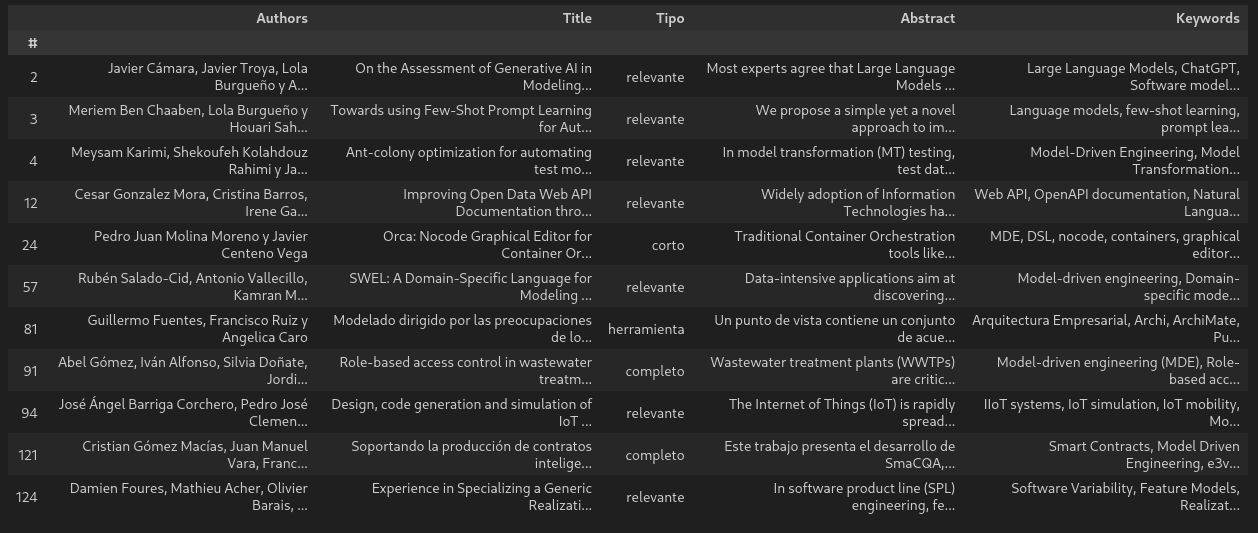
\includegraphics[width=\textwidth]{img/resumen}
\end{frame}

\begin{frame}
  \frametitle{Tipos de artículos}
  \centering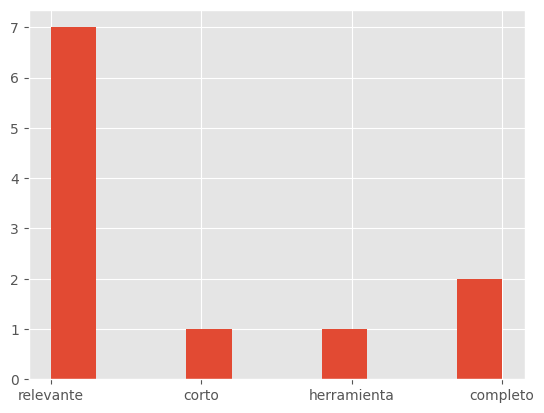
\includegraphics[height=.9\textheight]{img/histograma-tipos}
\end{frame}

\begin{frame}[fragile]
  \frametitle{Keywords}
\begin{lstlisting}
set(df['Keywords'].str.split(',').explode().str.strip())
>>> {'UML', 'Software models', 'Natural Language Generation', 'Ant Colony Optimization', 'Puntos de Vista', 'BPMN', 'Domain-specific modeling', 'ArchiMate', 'Archi', 'Smart Contracts', 'IIoT systems', 'Positive', 'Model Transformation Testing', 'Data-driven workflows', 'OpenAPI documentation', 'Artificial Intelligence', 'graphical editors', 'Software Variability', 'IoT mobility', 'Natural Language Processing', 'Automated Model Generation', 'Feature Models', 'Arquitectura Empresarial', 'Conceptual modeling', 'ChatGPT', 'IoT simulation', 'Model-driven development', 'DSL', 'Model-Driven Engineering', 'Business Modeling', 'Modeling languages', 'Language models', 'nocode', 'Realization Models', 'Data-intensive applications', 'domain modeling', 'model completion', 'MDE', 'Model-driven engineering (MDE)', 'Web API', 'containers', 'Model-to-text transformation', 'Wastewater treatment plant (WWTP)', 'few-shot learning', 'Docker', 'Model-driven engineering', 'Large Language Models', 'Role-based access control (RBAC)', 'Data science', 'e3value', 'prompt learning', 'Code generation', 'Negative Variability', 'Model Driven Engineering'}
\end{lstlisting}

\end{frame}


\begin{frame}[fragile]
  \frametitle{Número de autores}
\begin{lstlisting}[basicstyle=\large\tt]
len(df['Authors'].str.replace(' y ', ",",regex=False).str.split(',').explode().str.strip().unique())
>>> 43
\end{lstlisting}
\end{frame}


\begin{frame}
  \frametitle{Metamodelo del track}
\centering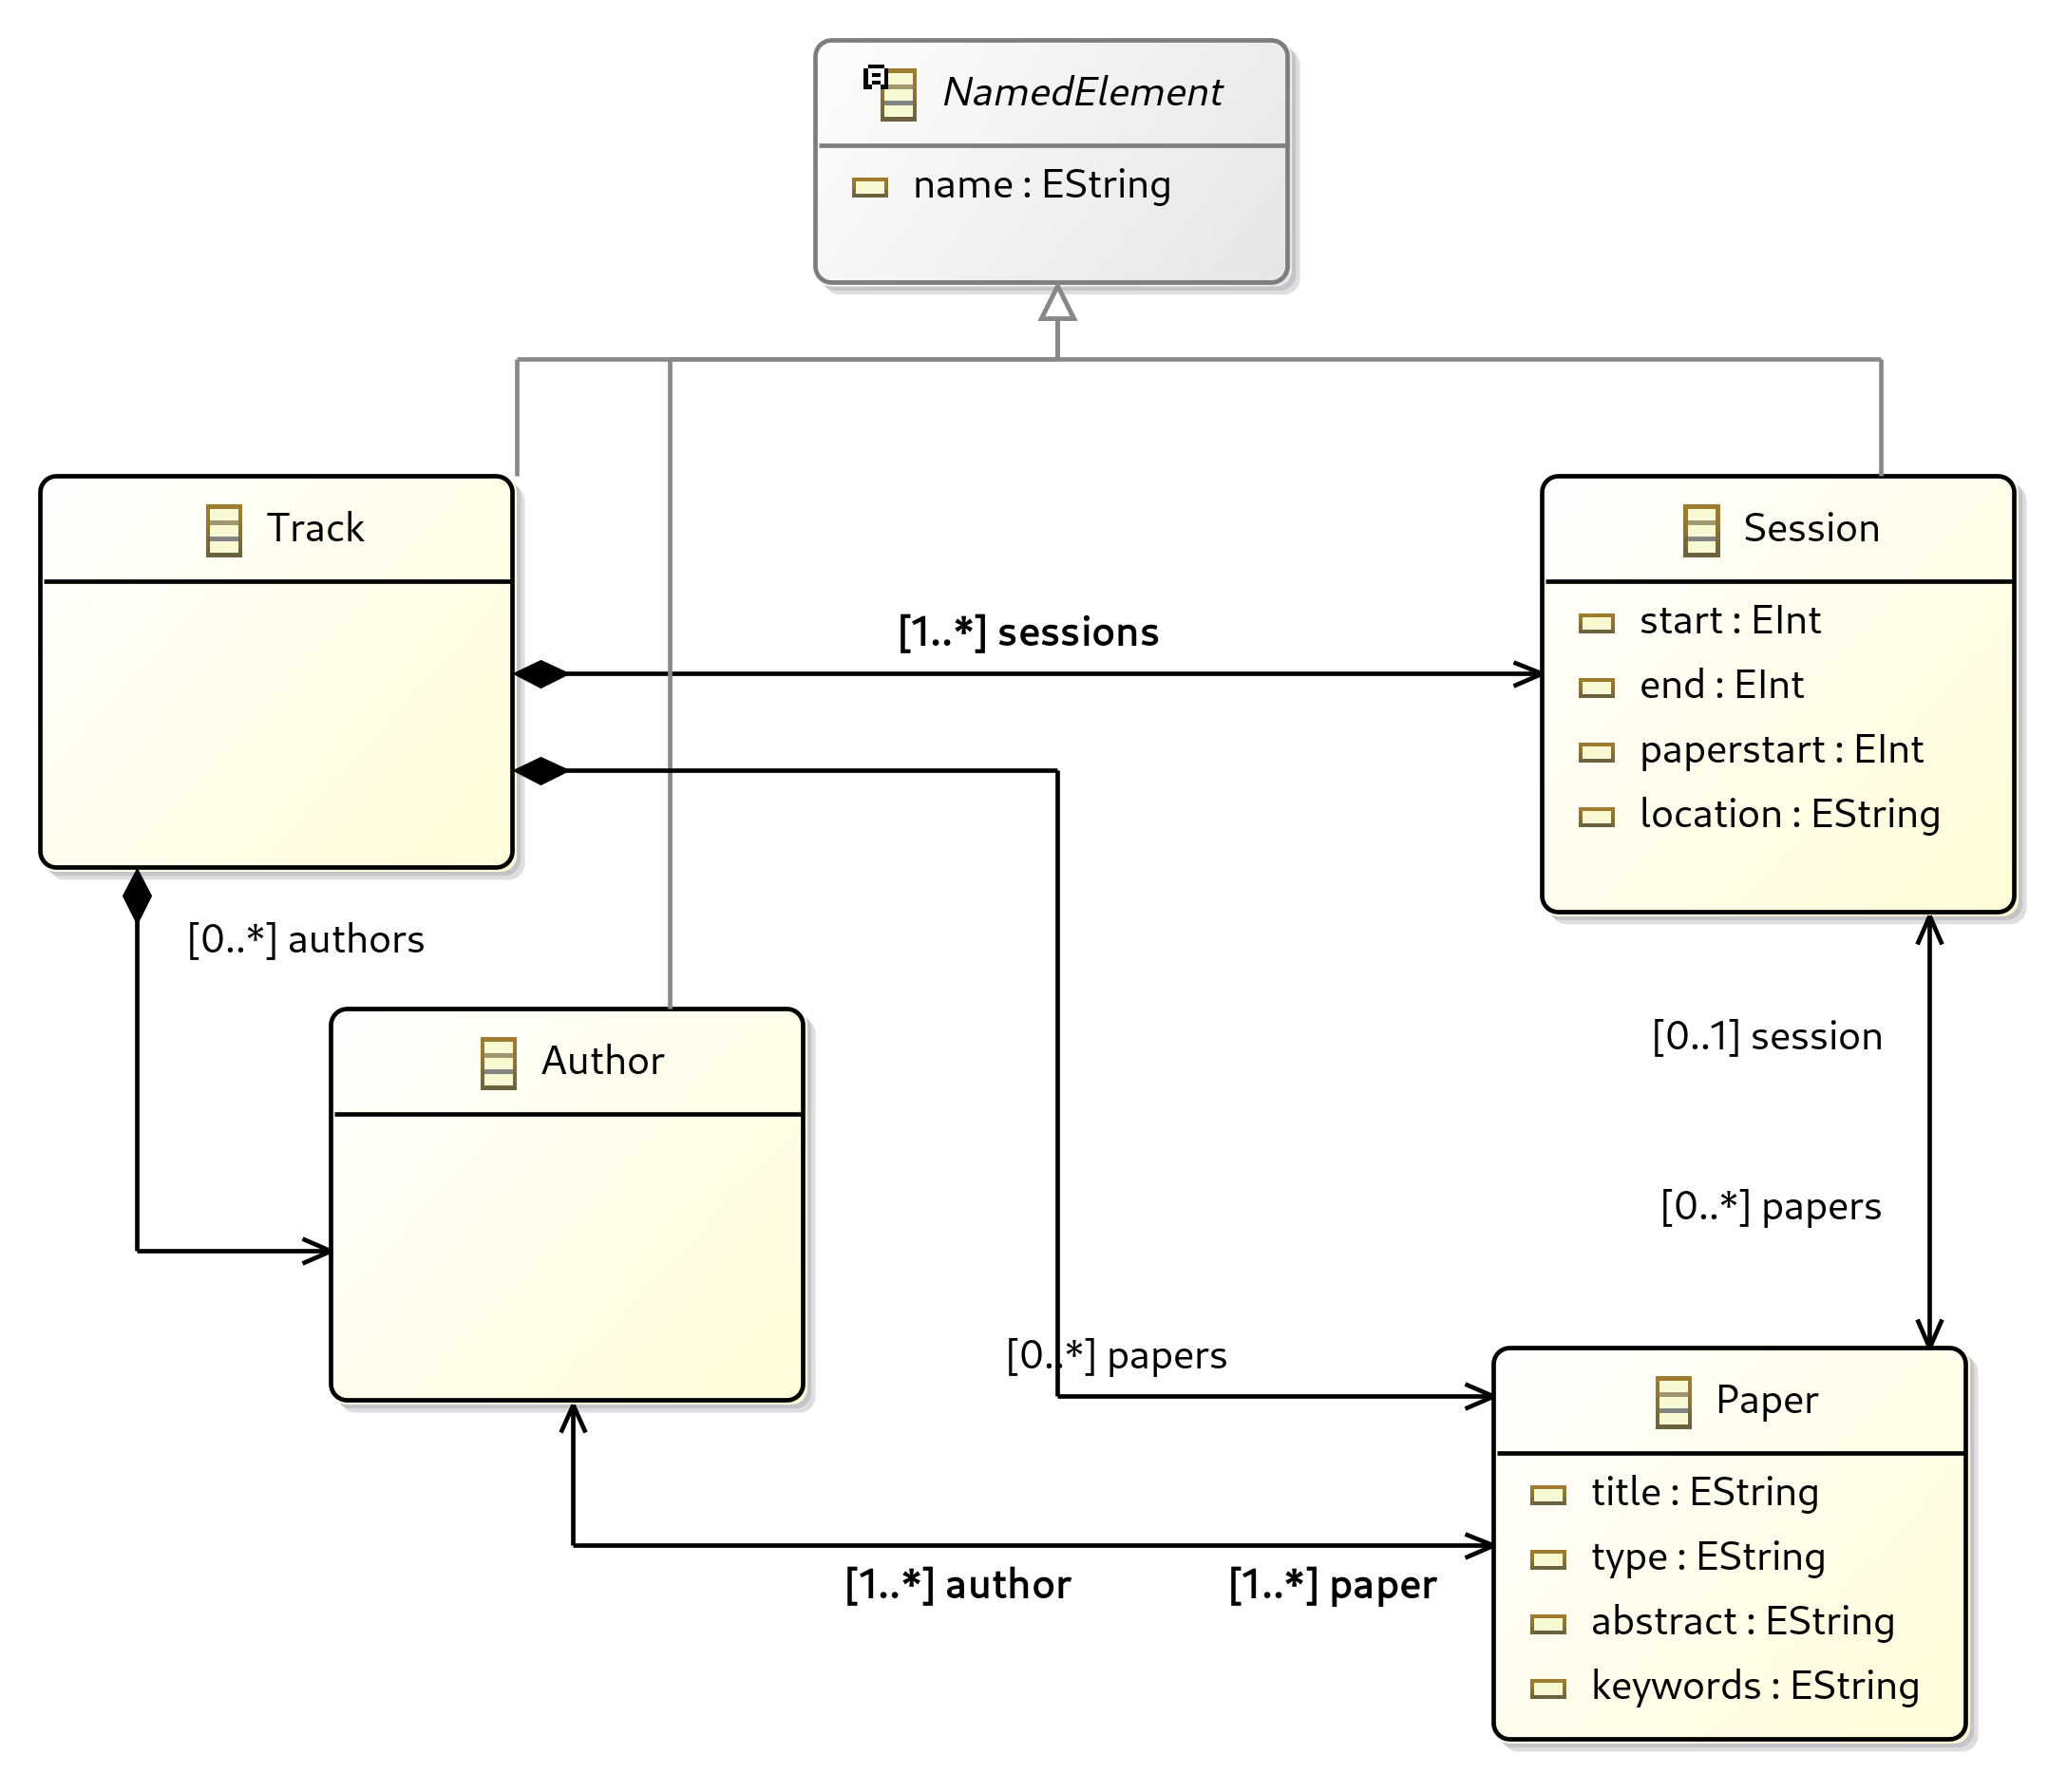
\includegraphics[height=.9\textheight]{img/IsdmTrack}
\end{frame}

\begin{frame}[fragile]
  \frametitle{PyEcore para construir el modelo}
\begin{lstlisting}[basicstyle=\large\tt]
%pip install pyecore pyecoregen
!pyecoregen -e IsdmTrack.ecore -o . --auto-register-package

import IsdmTrack as isdm

track = isdm.Track(name="ISDM'24")
for index, row in df.iterrows():
    paper = isdm.Paper(title=row['Title'],
                       type=row['Tipo'],
                       abstract=row['Abstract'],
                       keywords=row['Keywords'])

    track.papers.append(paper)
    ...
\end{lstlisting}
\end{frame}


\begin{frame}[fragile]
  \frametitle{Model-to-Text!!}
Renderizado:
\begin{lstlisting}
template = Template(open('templates/sessionslide-model.tex.j2').read())

for session in track.sessions:
    print(template.render(session=session))
\end{lstlisting}



  Plantilla {\tt sessionslide-model.tex.j2}:
\lstinputlisting[language=TeX]{../code/templates/sessionslide-model.tex.j2}
\end{frame}

\begin{frame}[fragile]
  \frametitle{Incluso, la cabra tira al monte... NoSQL con Neo4j}

\begin{lstlisting}
def add_papers(tx, papers: list[isdm.Paper]):
    for p in papers:
        tx.run(f"""CREATE (p:Paper) SET p.title = "{p.title}", p.type = "{p.type}", ...""")

def add_sessions(tx, sessions: list[isdm.Session]):
    for s in sessions:
        tx.run(f"""CREATE (s:Session) SET s.name = "{s.name}", s.start = "{s.start}", s.end = "{s.end}", ...""")

with GraphDatabase.driver(URI, auth=AUTH) as driver:
    with driver.session() as session:
        session.execute_write(add_papers, track.papers)
        session.execute_write(add_sessions, track.sessions)
\end{lstlisting}
\end{frame}

\begin{frame}
  \frametitle{Incluso, la cabra tira al monte... NoSQL con Neo4j}
  \centering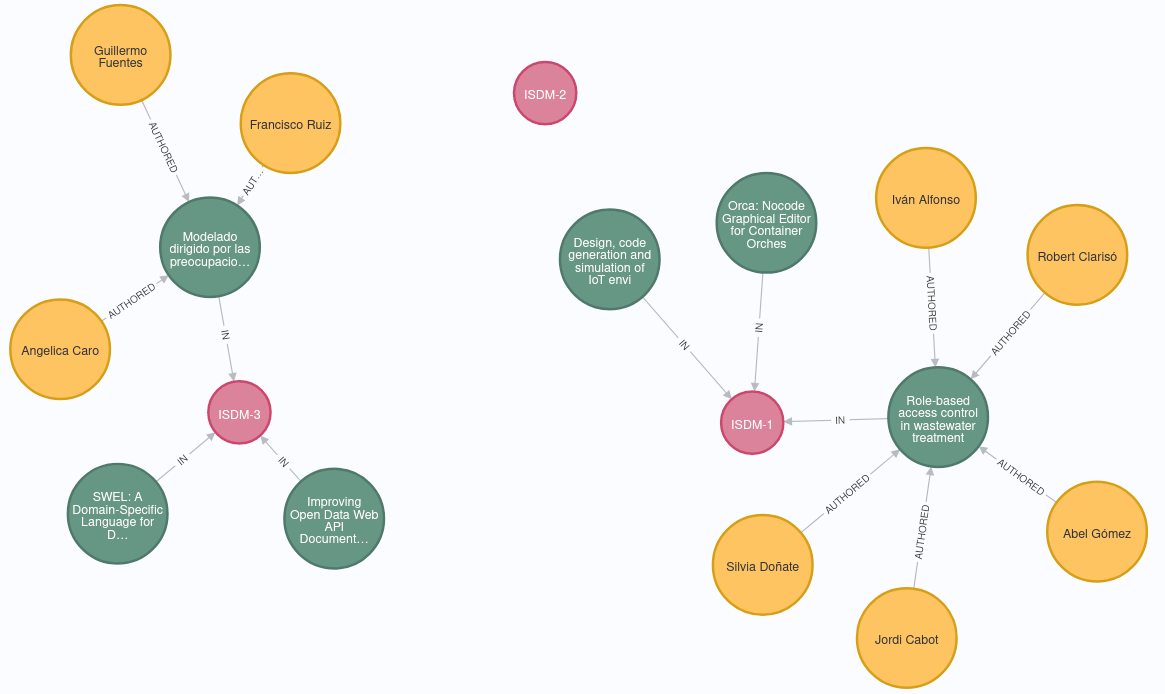
\includegraphics[height=.9\textheight]{img/sessions}
\end{frame}



\begin{frame}
  \frametitle{Y todos los artículos}
\centering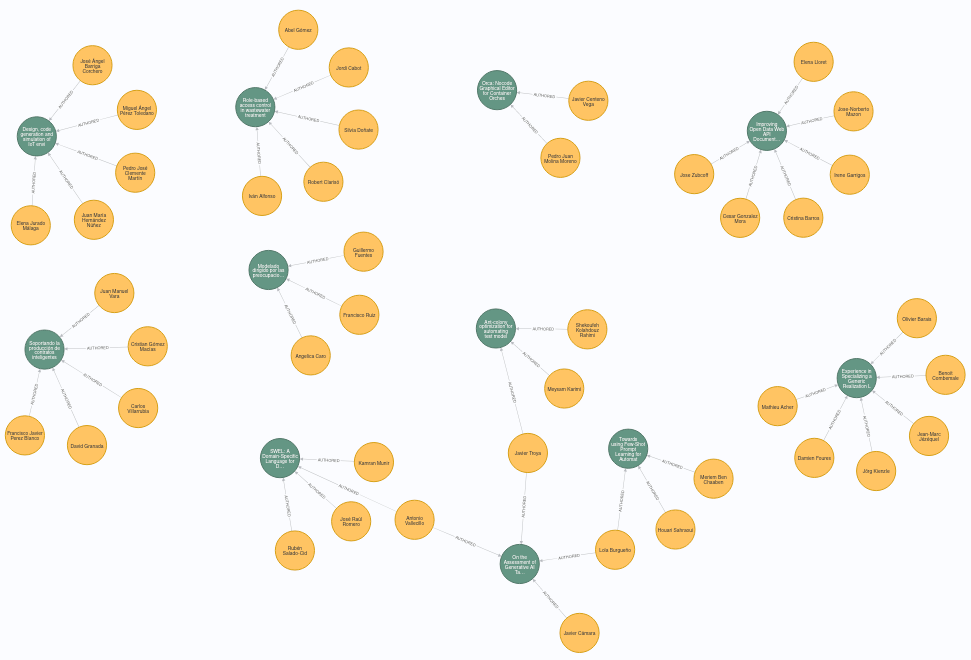
\includegraphics[height=.9\textheight]{img/papers}
\end{frame}


\input sessionindex


\end{document}

%%% Local variables:
%%% mode: LaTeX
%%% TeX-master: "header.tex"
%%% ispell-local-dictionary: "spanish"
%%% fill-column: 75
%%% TeX-parse-self: t
%%% TeX-auto-save: t
%%% End:
%%% vim: expandtab shiftwidth=2 tabstop=2 ai spelllang=es_ES spell tw=80

% LocalWords:  Extremadura
